\documentclass[journal,twoside,web]{ieeecolor}
\usepackage{jsen}
\usepackage{cite}
\usepackage{amsmath,amssymb,amsfonts}
\usepackage{algorithmic}
\usepackage{graphicx}
\usepackage{textcomp}
\usepackage{wrapfig}

% Added by S.Niespodziany
\usepackage{subcaption}
\usepackage{float}
\usepackage{booktabs}
\usepackage{multirow}


\def\BibTeX{{\rm B\kern-.05em{\sc i\kern-.025em b}\kern-.08em
    T\kern-.1667em\lower.7ex\hbox{E}\kern-.125emX}}
\markboth{\journalname, VOL. XX, NO. XX, XXXX 2024}
{Niespodziany \MakeLowercase{\textit{et al.}}: iFOG modulator design and optimization for maximizing scale factor control precision}
\definecolor{abstractbg}{rgb}{0.89804,0.94510,0.83137}
\setlength{\fboxrule}{0pt}
\setlength{\fboxsep}{0pt}

\begin{document}
\title{iFOG modulator design and optimization for maximizing scale factor control precision}
\author{Sławomir Niespodziany
    % \thanks{This paragraph of the first footnote will contain the date on
    %     which you submitted your paper for review. It will also contain support 
    %     information, including sponsor and financial support acknowledgment. For 
    %     example, ``This work was supported in part by the U.S. Department of 
    %     Commerce under Grant BS123456.'' }
    % \thanks{The next few paragraphs should contain
    %     the authors' current affiliations, including current address and e-mail. For 
    %     example, F. A. Author is with the National Institute of Standards and 
    %     Technology, Boulder, CO 80305 USA (e-mail: author@boulder.nist.gov). }
    % \thanks{S. B. Author, Jr., was with Rice University, Houston, TX 77005 USA. He is
    %     now with the Department of Physics, Colorado State University, Fort Collins, 
    %     CO 80523 USA (e-mail: author@lamar.colostate.edu).}
    % \thanks{T. C. Author is with
    %     the Electrical Engineering Department, University of Colorado, Boulder, CO 
    %     80309 USA, on leave from the National Research Institute for Metals, 
    %     Tsukuba, Japan (e-mail: author@nrim.go.jp).}
}

\IEEEtitleabstractindextext{%
    \fcolorbox{abstractbg}{abstractbg}{%
        \begin{minipage}{\textwidth}%
            % \begin{wrapfigure}[12]{r}{3in}%
            %     
\includegraphics[width=3in]{jsenga.png}%
            % \end{wrapfigure}%
            \begin{abstract}
                This paper presents the design and optimization of a modulator subsystem for closed-loop interferometric fibre optic gyroscopes, with a focus on maximizing scale factor control precision through an all-digital hardware architecture. The operating principle of the gyroscope is reviewed, followed by a description of the four-step modulation scheme used to linearize the optical response, maintain maximum sensitivity, and enable rotation direction detection. Two modulator architectures are analyzed and compared: a mixed analog-digital design employing a dedicated programmable gain stage, and a fully software-defined all-digital implementation. The all-digital approach is advocated for its reduced component count, fewer nonlinearity sources, and greater flexibility during development. A mathematical analysis of quantization error is derived to characterize the achievable scale factor control accuracy as a function of digital-to-analog converter resolution and reference voltage selection. The derivation reveals that the scale factor feedback signal depends on four consecutive drive samples rather than two, a non-obvious result with direct consequences for algorithm correctness. Based on this analysis, common implementation pitfalls are identified and discussed, including insufficient sample history, drive asymmetry due to discrete amplitude representation, and resolution loss caused by symmetric rounding of signed values. An optimal algorithm is presented, utilizing fixed-point arithmetic with concrete rounding method to recover one bit of effective resolution relative to naive implementations. The results establish a software foundation for high-precision closed-loop interferometric fibre optic gyroscope modulator design.
            \end{abstract}
            
            \begin{IEEEkeywords}
                all-digital modulator, fibre optic gyroscope, fixed-point arithmetic, four-step modulation, scale factor control, Sagnac effect.
            \end{IEEEkeywords}
        \end{minipage}}}
\maketitle

\section{Introduction}
\label{sec:introduction}
iFOG (Interferometric Fibre Optic Gyroscope) concept is based on the Sagnac effect \cite{post1967sagnac}, discovered in 1913 \cite{sagnac1913ether}. Over the years, the design has has been excercised multiple times. However, the limits which hold the development back are constantly pushed forward as technology evolves. This allows for better precision, miniaturized size, lower power consumption, etc. At the same time, the ever progressing industry finds new and more strict applications for the gyroscopes, setting the requirements bar even higher. Such a context makes the already existing designs being tested and optimized in every possible aspect. This applies equally to all the optical and electro--optic componenents, the electronics and the driving software. A crucial part of the control system of an iFOG is the modulator. In a closed--loop design \cite{pavlath1996closed} it is a vital element of the feedback loop. It directly affects the overall performance. It drives the optical circuit into a predefined state, in which the circuit's response can be demodulated and error signals determined. Modulator accuracy has critical impact on the resulting performance. This paper takes a closer look at the all--digital implementation of the modulator subsystem - in particular on its electronic architecture and the algorithm controlling it. Mathematical analysis is conducted to allow for pure--software optimization of algorithm's accuracy.

\section{Principle of operation - open--loop configuration}
Light source of an iFOG generates a light beam, which is ideally split in 50/50 ratio. Each half enters a loop of relatively long fiber through each of its ends. The fiber length $L$ determines light transit time $\tau$ through it - Equation~\ref{eq:transit_time}, where $n$ is the refraction coefficient, affecting light speed in the medium.

\begin{equation}
    \tau = \frac{L}{n \cdot c}
    \label{eq:transit_time}
\end{equation}

\noindent
The halves go past each other and exit on the opposite ends of the fiber. The optical circuit is arranged, so that the two exitting beams interfere with each other and the resulting light intensity is measured by a detector. When the circuit stays at rest, the beams interfere with zero phase shift ($\Delta\phi = 0$), resulting in maximum intensity $P_0$ measured at the detector. However, when the loop rotates, the two halves travel paths of a slightly different length, resulting in non--zero phase shift. The relative phase shift at the interference point is rotation dependent and in this paper it is reffered to as the Sagnac--induced phase shift

\begin{equation}
    \Delta\phi_s = \frac{2\pi \cdot L  \cdot D \cdot n}{\lambda \cdot c} \cdot \omega
    \label{eq:phase_shift}
\end{equation}

\noindent
where $D$ - fiber loop diameter, $\omega$ - angular velocity, $\lambda$ - wavelength.

\noindent
This has been depicted in Figure~\ref{fig:fog}. Both halves enter the loop at the \textit{entry point}. After the transit time they exit through the same point - now an \textit{exit point}. Because of the non--zero rotation, this point moves along the loop, effectively shrinking one path and extending the other. Path difference is relatively small, thus it is expressed as a phase difference in wavelength domain.

\begin{figure}[ht]
    \centering
    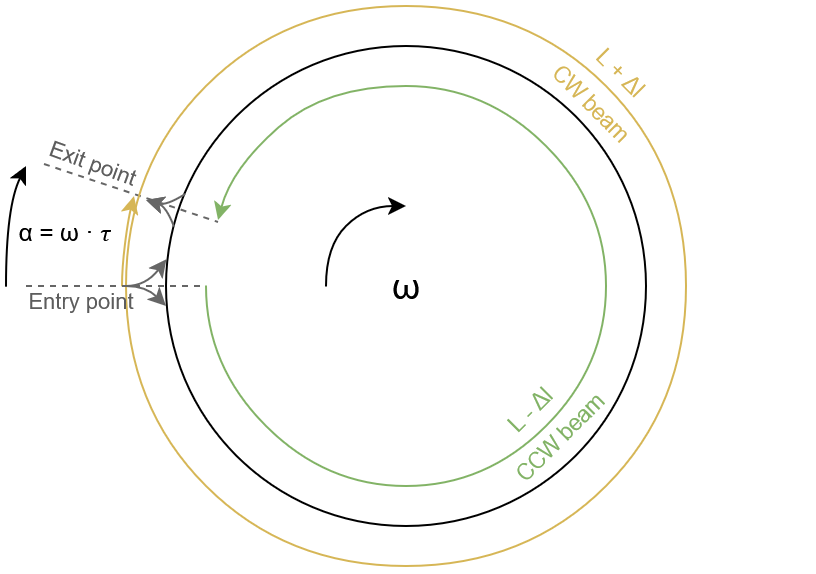
\includegraphics[width=204px]{img/fog.png}
    \caption{Two counterpropagating light beam halves enter the fiber loop at the \textit{Entry point}. Their phase is initially in sync. After transit time $\tau$ they exit and interfere. During that time the \textit{Entry/Exit point} moves according to the rotation rate $\omega$ (by the angle $\alpha = \omega \cdot \tau$). As a result the CW and CCW halves cover non--equal path lengths ($L\pm\Delta{}l$), which leads to a non--zero phase difference.}
    \label{fig:fog}
\end{figure}

\noindent
The formula in Equation~\ref{eq:response}, also presented in Figure~\ref{fig:response}, is the optical circuit response function \cite{babu2016digital}. It describes how the measured light intensity depends on the total phase shift of the interfering light.

\begin{equation}
    P(\Delta\phi) = \frac{P_0}{2} \cdot (1 + cos(\Delta\phi))
    \label{eq:response}
\end{equation}

\begin{figure}[ht]
    \centering
    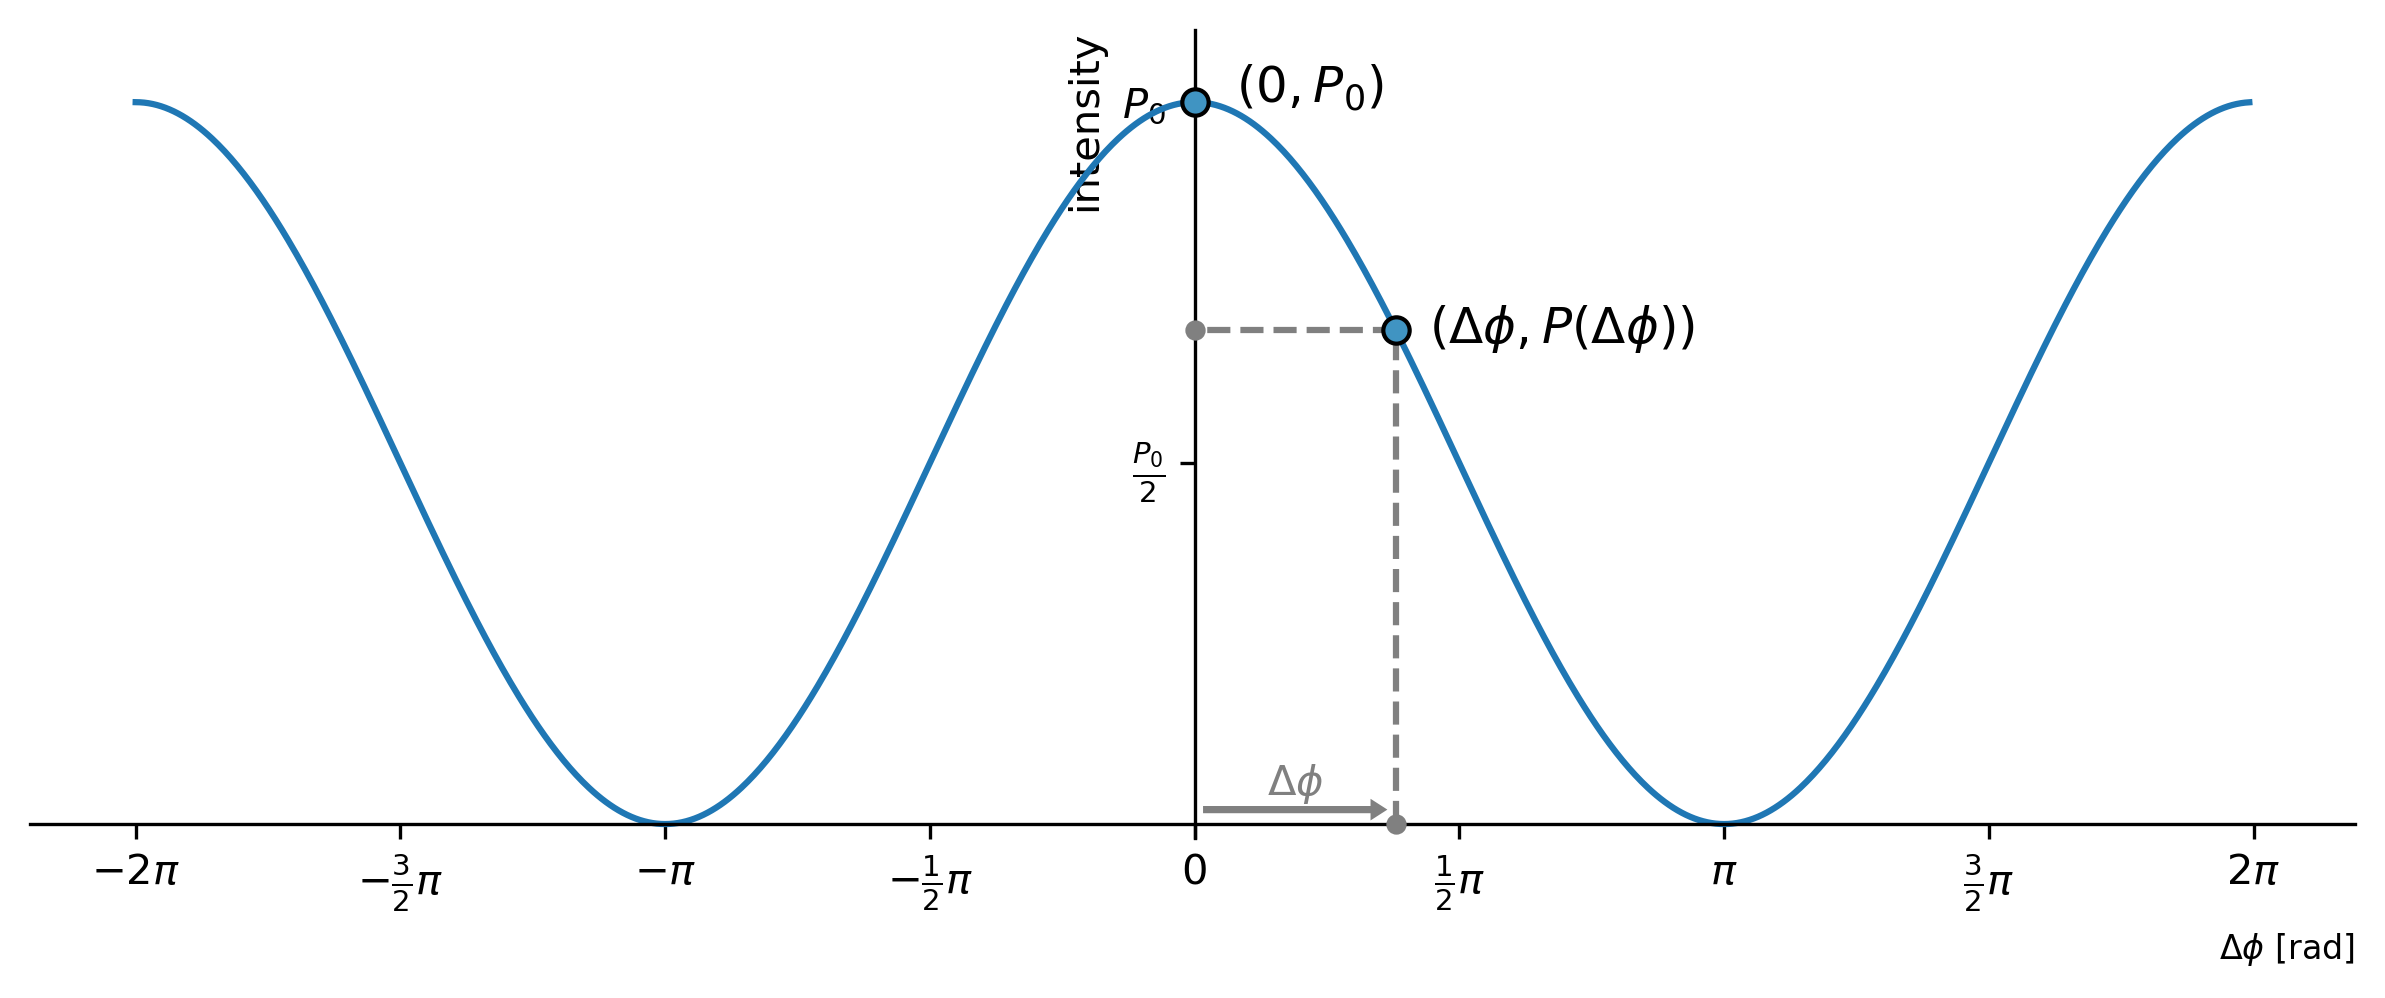
\includegraphics[width=1.0\linewidth]{img/response.png}
    \caption{Optical circuit response is an upshifted cosine. The two exemplary operating points refer to the circuit being at rest, yielding the maximum possible intensity in $(0, P_0)$ and a circuit subjected to rotation, at non--zero phase shift and decreased intensity in $(\Delta\phi, P(\Delta\phi))$.}
    \label{fig:response}
\end{figure}

\noindent
When the circuit is at rest ($\omega = 0 \rightarrow \Delta\phi = 0$), the operating point resides at peak intensity $P_0$. A non--zero rotation results in phase shift moving the operating point according to rotation rate and its direction, decreasing the measured intensity. Two problems are linked with this \textit{open--loop} operation \cite{lefevre1993fiber}. Firstly, intensity drop alone does not allow for determining rotation direction - response function is symmetrical. Secondly, in the resting region, the slope is flat, thus the sensitivity is zero. With greater rotation rate, the slope becomes more steep, reaching its maximum sensitivity in $\Delta\phi = \pm\frac{\pi}{2}$, but then decreases again. For these reasons a \textit{closed--loop} configuration is superior in performance.

\section{Modulation scheme - closed--loop configuration}
In a closed--loop configuration \cite{lefevre1993fiber} the control system biases optical circuit sequentially in four predefined points $\Delta\phi \in \{+\frac{3}{2}\pi, -\frac{1}{2}\pi, -\frac{3}{2}\pi, +\frac{1}{2}\pi\}$, utilizing the \textit{four--step} modulation \cite{wang2012method} (Figure~\ref{fig:bias}). This allows for linearizing the response, keeping the circuit at maximum sensitivity and detecting rotation direction.

\begin{figure}[ht]
    \centering
    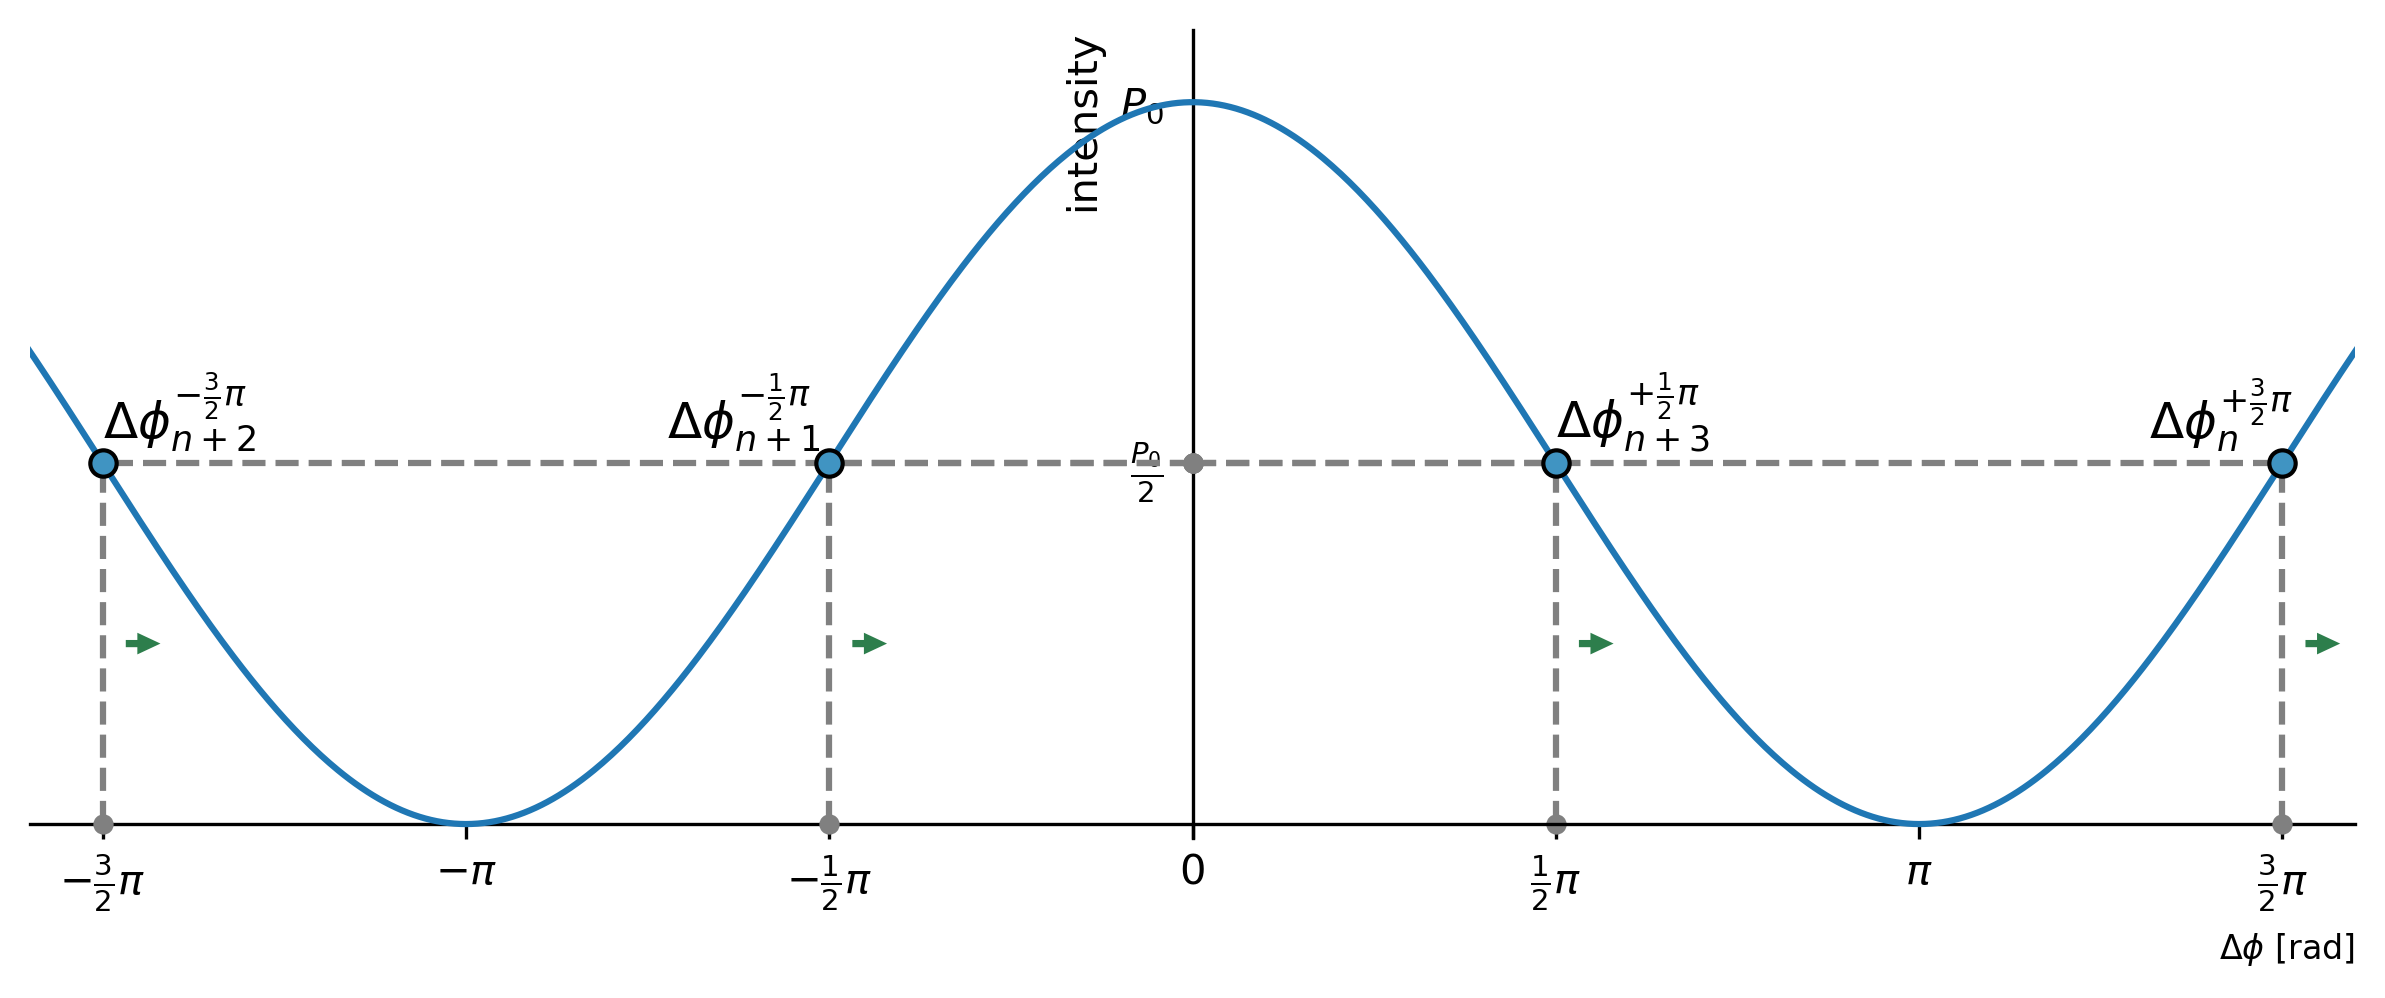
\includegraphics[width=1.0\linewidth]{img/bias.png}
    \caption{Circuit biased in four points of highest sensitivity.}
    \label{fig:bias}
\end{figure}

Compared to \textit{two--step} modulation \cite{wang2012method} this scheme is supreme, as it allows for controlling the \textit{scale factor} - an essential parameter for maintaining device performance. Modulator injects the mentiobned phase shifts by using an electro--optic actuator placed on the fiber path. The amount of applied shift is controlled by an electronic circuit. It performs digital calculations and generates corresponding voltages via a digital--to--ananlog converter and an electronic front--end. The voltage is translated to a phase shift according to the half--wave voltage $V_\pi$ - a parameter of the actuator. Each element in this pipeline is a subject to temperature drift and aging \cite{salvestrini2011analysis} effects, which influence the total combined gain. For this reason, continous calibration is required for maintaining measurement accuracy and it is realized by tracking the scale factor. This allows the control algorithm to know where the desired bias points are in the digital domain, while they constantly drift.

Diagrams in Figure~\ref{fig:bias_errors} depict how the biased circuit responds to various conditions - i.e. misaligned scale factor and uncompensated rotation present. While this paper does not discuss in details how the rotation is measured, it is crucial to emphasize, that different feedback signals can be derived for scale factor adjustment and rotation measurement. These feedback signals allow the digital control loop for adjusting runtime parameters and placing the operating points exactly where they are intended to be.

\begin{figure}[H]
    \centering
    \begin{subfigure}[b]{0.48\textwidth}
        \centering
        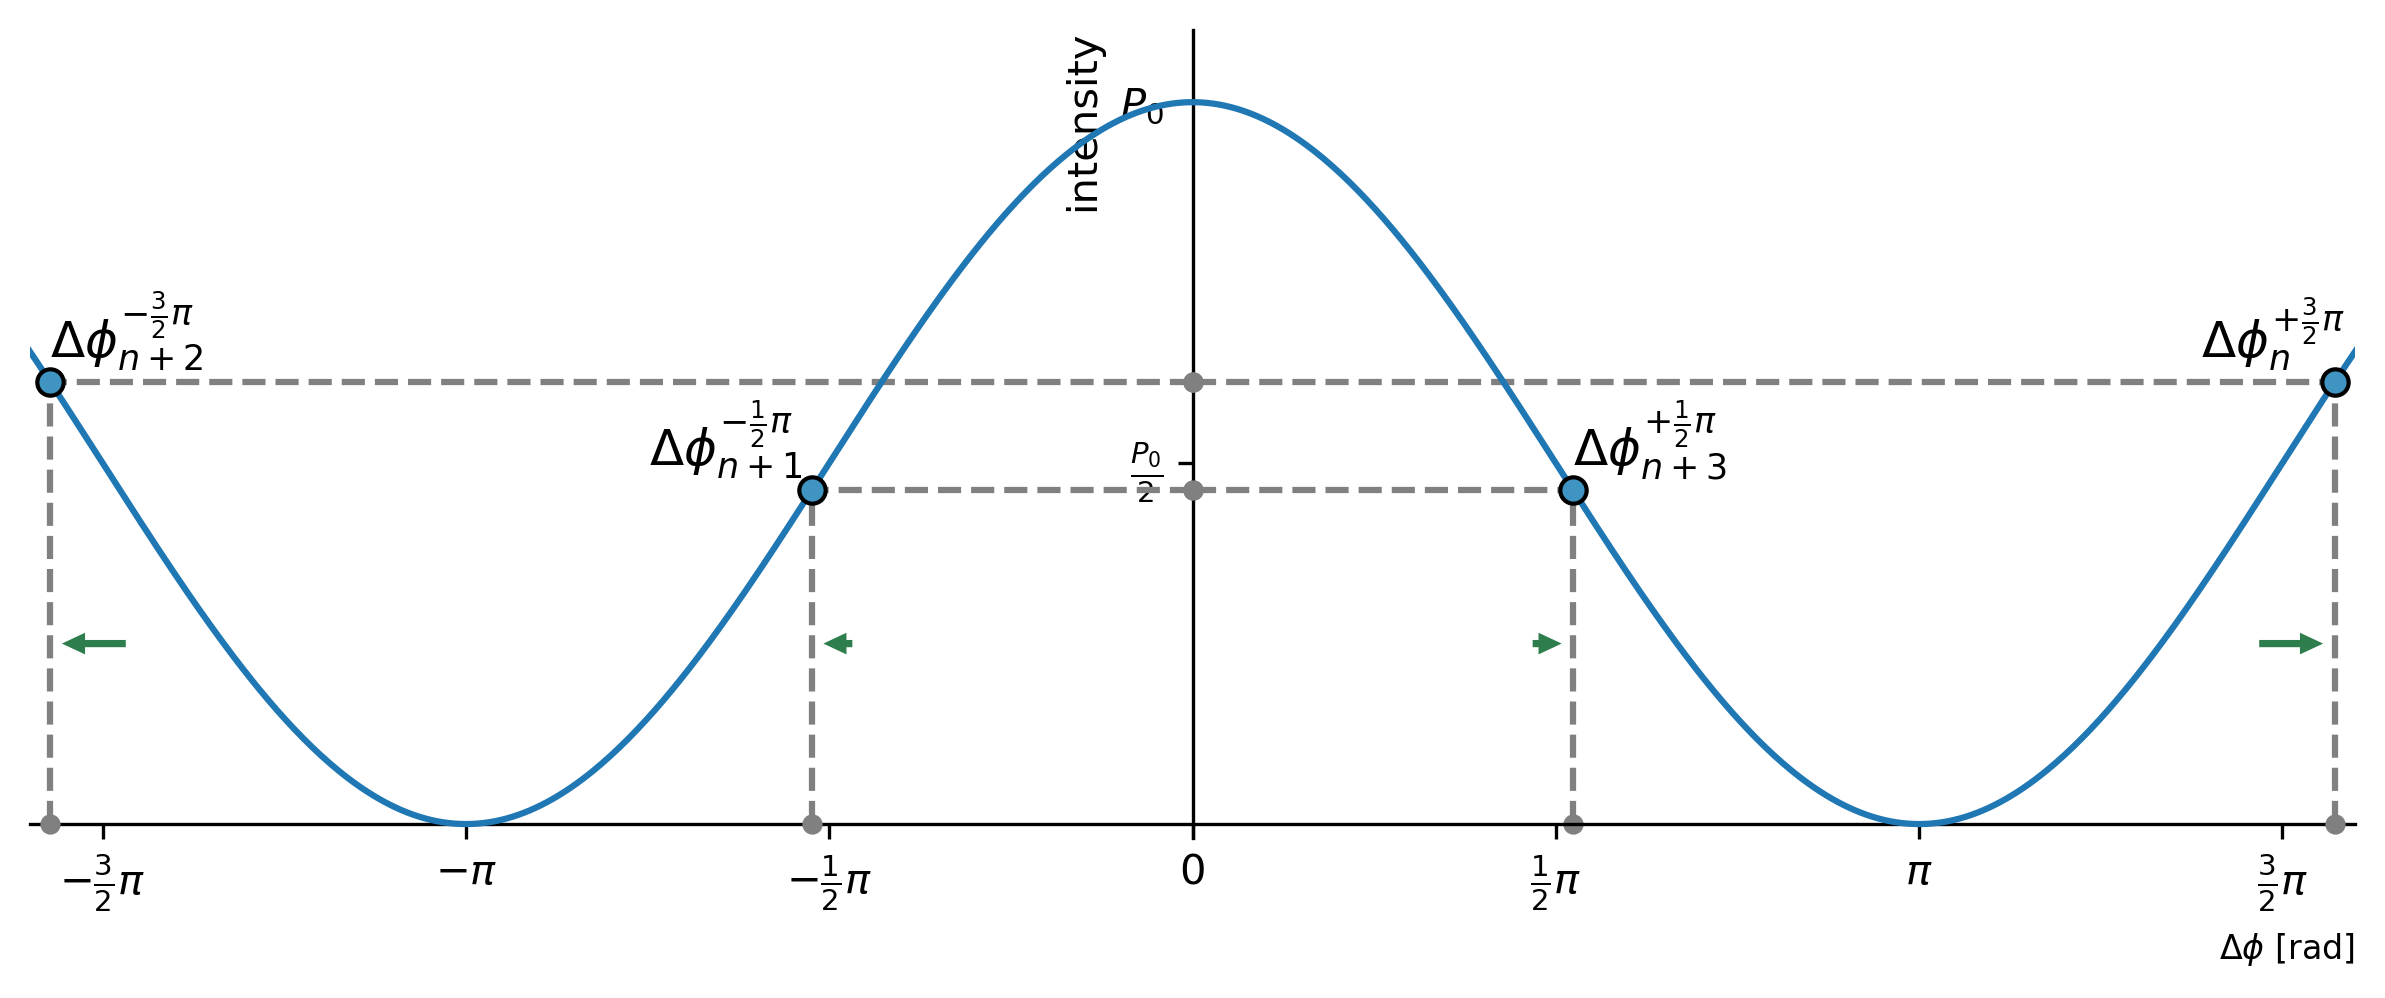
\includegraphics[width=\textwidth]{img/bias_factor_high.png}
        \caption{Scale factor too high - bias points are shifted away from zero, resulting in intensity imbalance.}
        \label{fig:bias_factor_high}
    \end{subfigure}
    \begin{subfigure}[b]{0.48\textwidth}
        \centering
        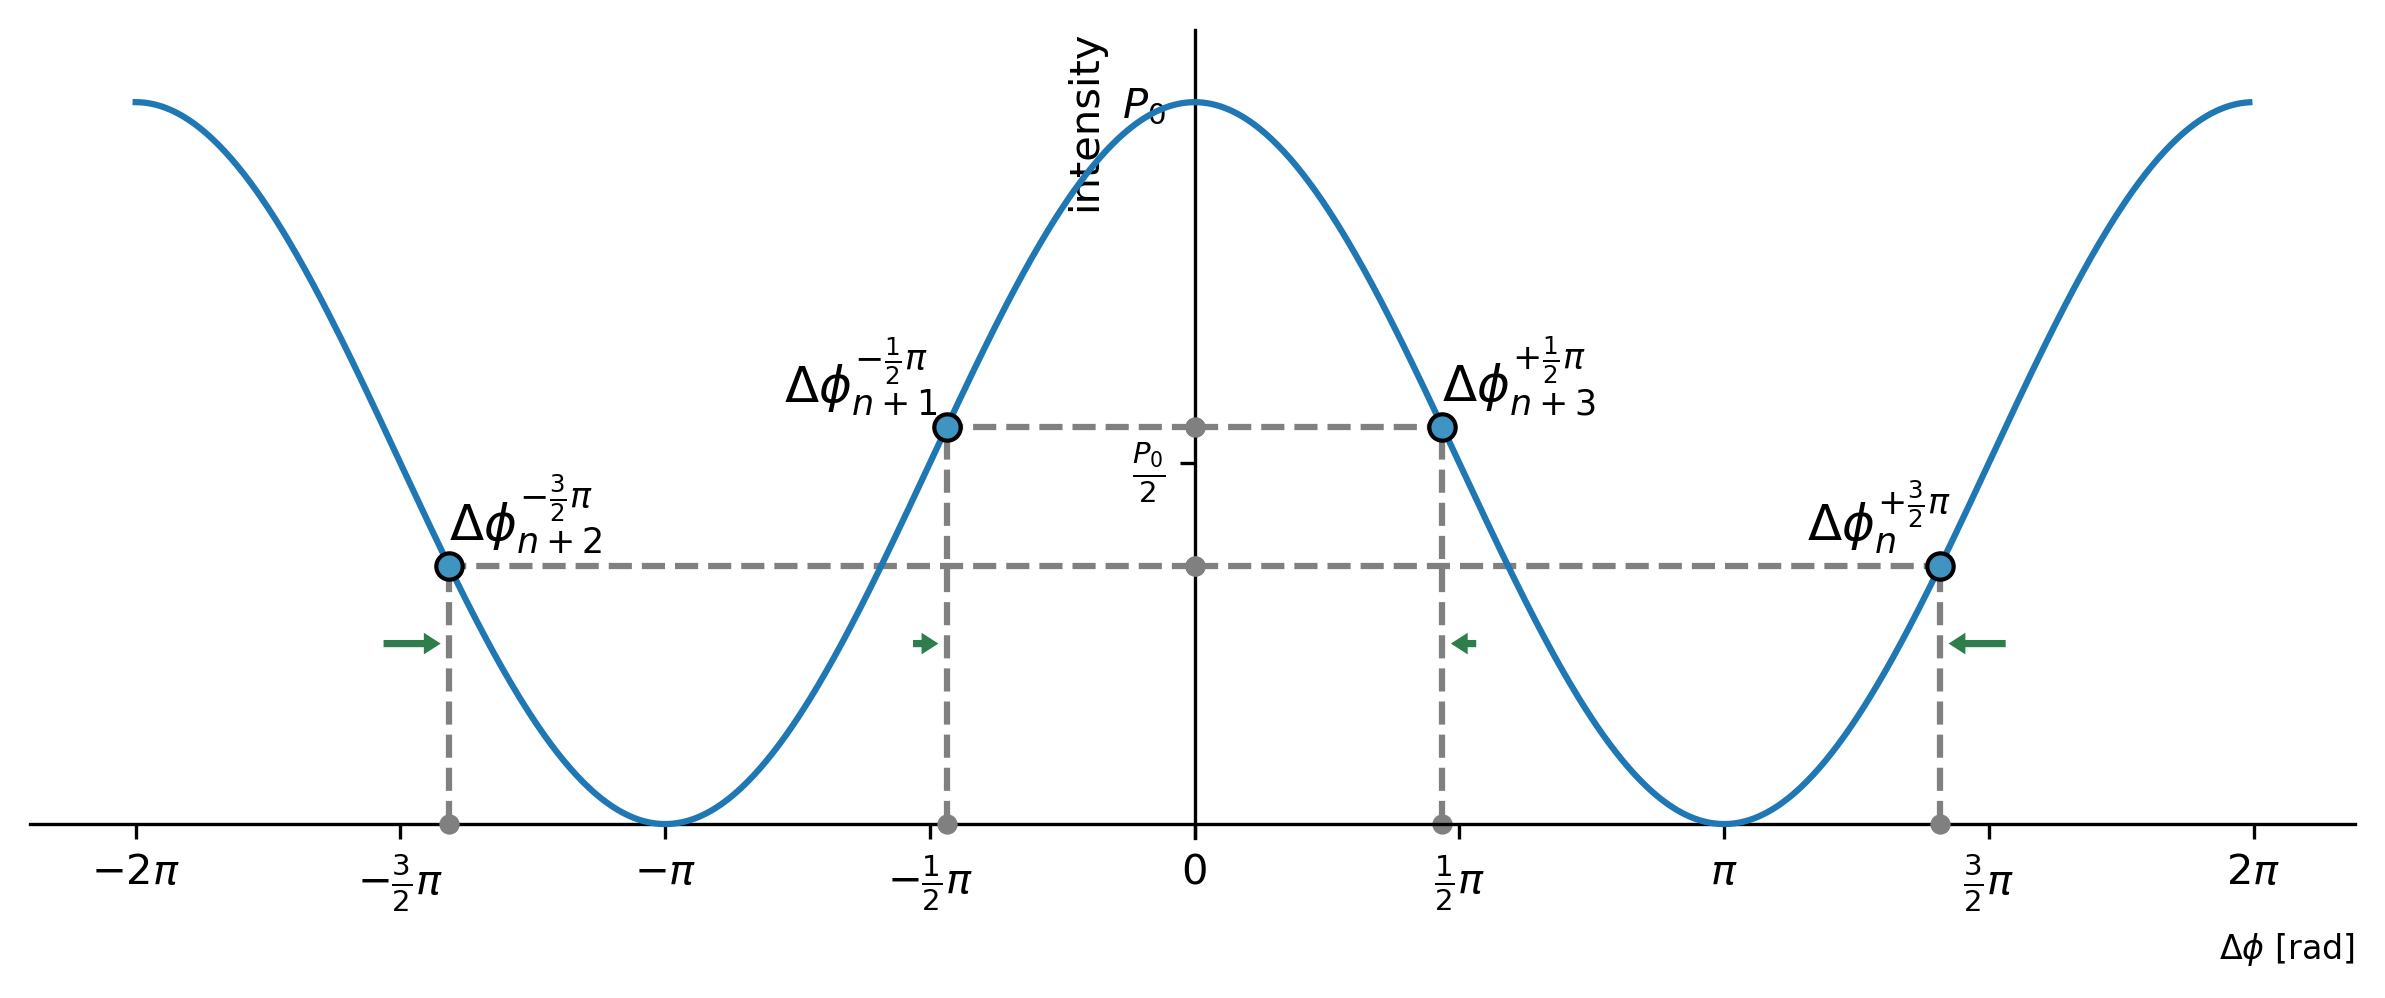
\includegraphics[width=\textwidth]{img/bias_factor_low.png}
        \caption{Scale factor too low - bias points shifted towards zero, resulting in opposite imbalance.}
        \label{fig:bias_factor_low}
    \end{subfigure}
    \begin{subfigure}[b]{0.48\textwidth}
        \centering
        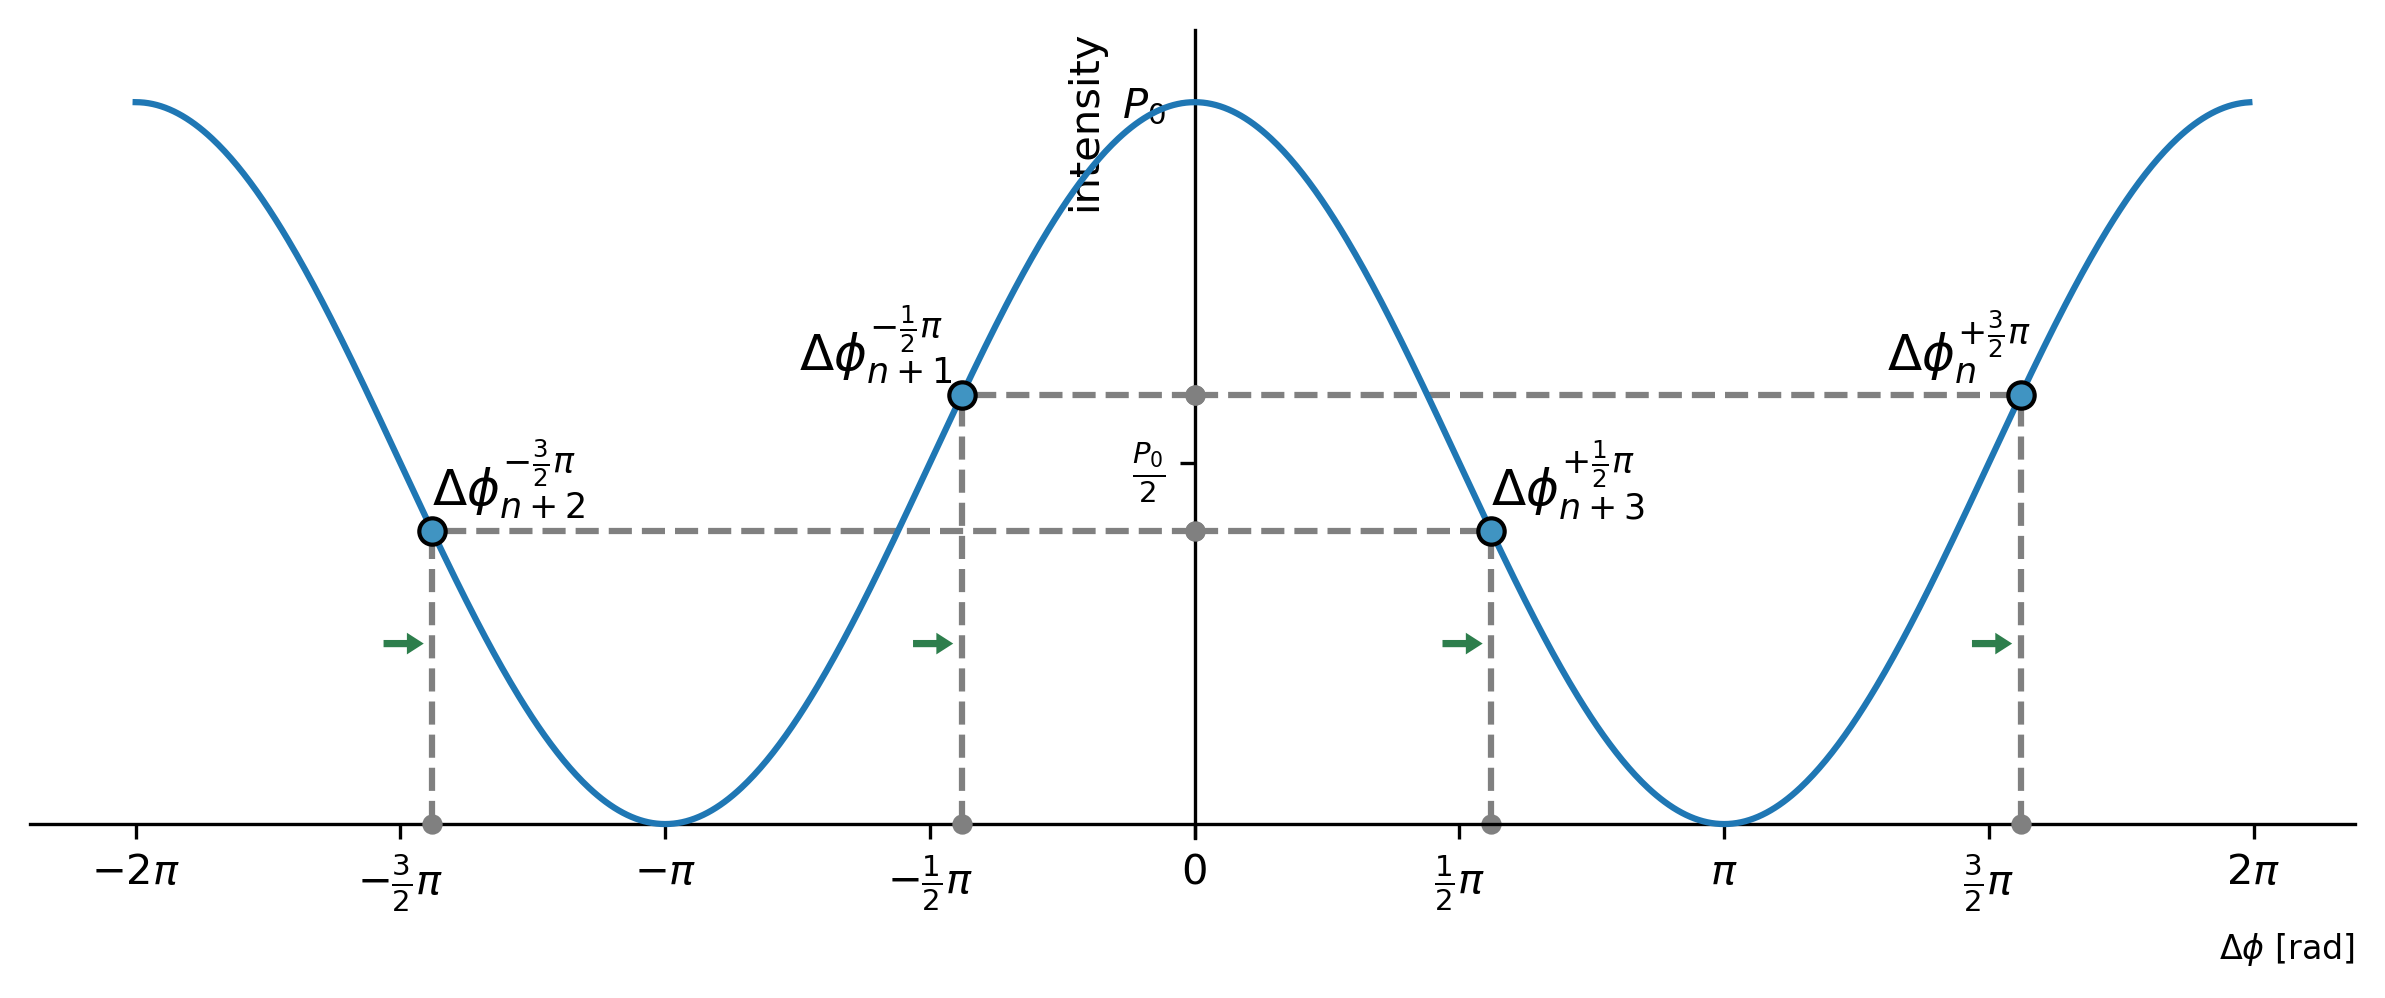
\includegraphics[width=\textwidth]{img/bias_shift_pos.png}
        \caption{Phase shift induced by positive rotation - bias points shifted right. Points $\{4n, 4n+1\}$ result in higher intensity than points $\{4n+2, 4n+3\}$.}
        \label{fig:bias_shift_pos}
    \end{subfigure}
    \begin{subfigure}[b]{0.48\textwidth}
        \centering
        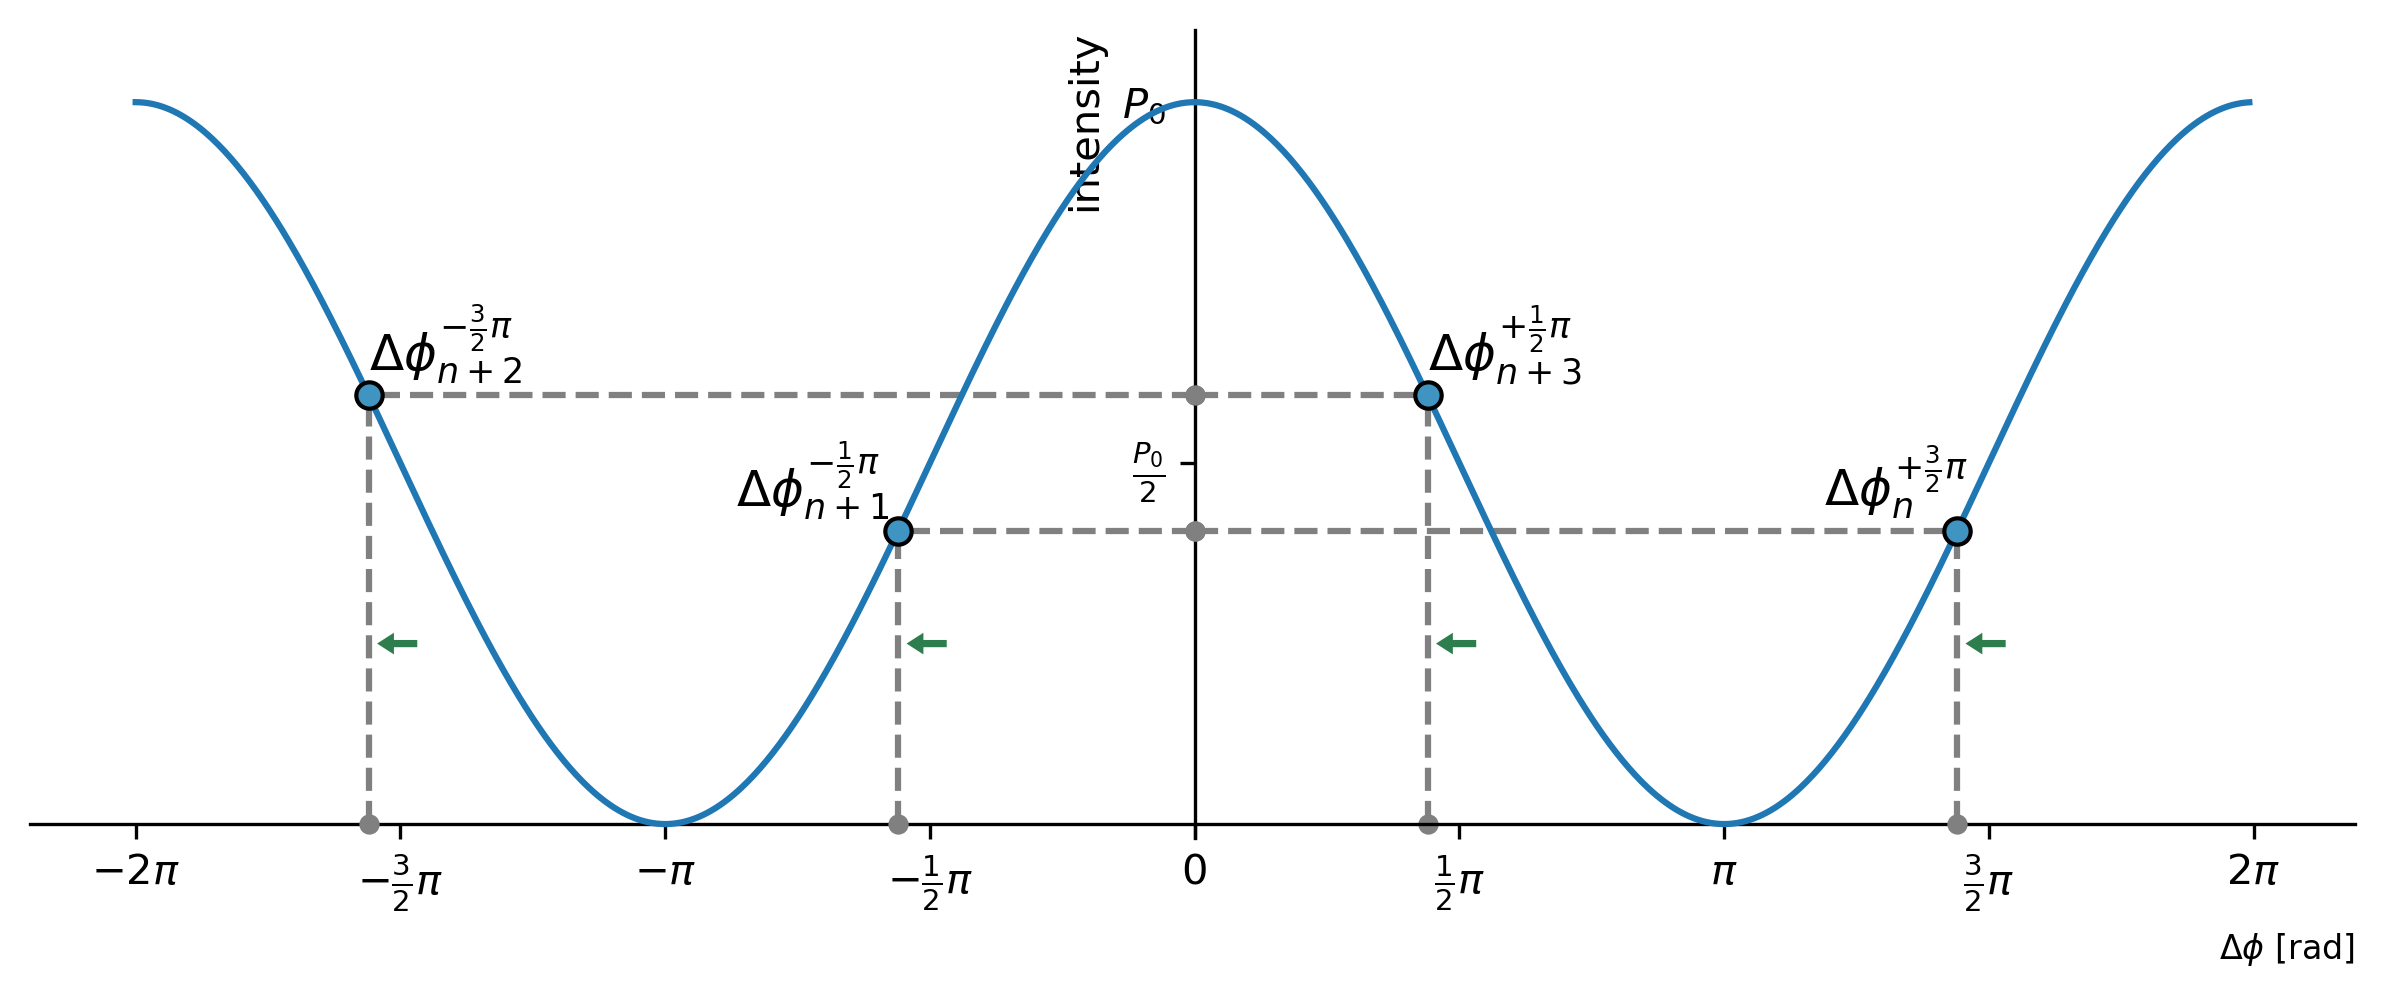
\includegraphics[width=\textwidth]{img/bias_shift_neg.png}
        \caption{Phase shift induced by negative rotation - bias points shifted left. Points $\{4n, 4n+1\}$ result in lower intensity than points $\{4n+2, 4n+3\}$.}
        \label{fig:bias_shift_neg}
    \end{subfigure}
    \caption{
        Four--step modulation allows for detection of scale factor error and uncompensated Sagnac--induced phase shift.}
    \label{fig:bias_errors}
\end{figure}

\textbf{TODO FIX IN THE FIGURE n+1 => 4n+1 etc.}

From control point of view and for simplicity, the combined scale factor can be reffered to as the half--wave voltage $V_{\pi}$. Even though the actuator gain drift is only one of the scale factor components, the assumed linearity of others, makes it convenient to aggregate all into a single parameter. Other, non--linear errors, such as DAC INL are out of scope of this analysis. The control system uses the combined scale factor to bias the optical circuit continously with the following bias point order:

\begin{equation}
    \begin{split}
        \{ & \Delta\phi_{4n+0}^{+\frac{3}{2}\pi} \rightarrow (+\frac{3}{4}\pi),    \\
           & \Delta\phi_{4n+1}^{-\frac{1}{2}\pi} \rightarrow (-\frac{1}{4}\pi),    \\
           & \Delta\phi_{4n+2}^{-\frac{3}{2}\pi} \rightarrow (-\frac{3}{4}\pi),    \\
           & \Delta\phi_{4n+3}^{+\frac{1}{2}\pi} \rightarrow (+\frac{1}{4}\pi) \}
    \end{split}
    \label{eq:bias_order}
\end{equation}

\noindent
where the superscripted phase is the intended effective phase shift for the given sample.

Modulator runs with the period of half the transit time $\frac{\tau}{2}$. This allows for the effective phase shift to be a result of a relative difference between every $k$'th and $(k-2)$'th samples. In such case the phase shift applied by the modulator for each sample can be half of the desired amplitude, reducing the overall required voltage range \cite{lefevre1993fiber}. Additionally, to null the effect of Sagnac--induced phase shift, modulator adds an ever--updating ramp signal, utilizing Serrodyne modulation \cite{pavlath1996closed} with the increment value of $\Delta\phi_r = -\Delta\phi_s$ - a phase shift of equal amplitude, but opposite sign. This way the algorithm nulls out the Sagnac--induced shift, while knowing how much of it it has cancelled, thus knowing the exact rotation rate. In every cycle, the software monitors both feedback signals and adjusts control accordingly.

\section{Modulator hardware architecture}
This paper opts in for an all--digital modulator architecture. Three distinct approaches can be distinguished:
\begin{enumerate}
    \item fully-analog, \label{arch:analog}
    \item mixed - digital with analog front end, \label{arch:mixed}
    \item all--digital. \label{arch:digital}
\end{enumerate}

\noindent
Firstly - a fully analog variant (\ref{arch:analog}), while feasible, does not comply with todays standards, where information is processed in a digital form. For integration with external systems, an analog--to--digital interface needs to be present anyway. In such case, incorporating an MCU or DSP in the processing loop brings the advantage of performing certain operations on pure data, rather than on signals carrying these data. A modern solution shall consist of a digital part for performing mathematical operations and electronic part for interfacing with the optical circuit - this resembles a classical - mixed - implementation (\ref{arch:mixed}). It consists of a DAC converter and a dedicated gain stage. Lastly, in a world of \textit{software--defined} solutions \cite{ulversoy2010software}, \cite{liu2022impact}, an architecture with the minimum possible amount of electronic components can be tempting. The two latter concepts are described in this section. The all--analog architecture will not be discussed.

\subsection{Dedicated gain stage}
A reasonable tradeoff between analog and digital approaches is the architecture proposed in \cite{lefevre1993fiber}. It is composed of a digital part - a DAC - and a dedicated analog gain stage. It has been depicted in Figure~\ref{fig:dedicated_gain_stage}.

\begin{figure}[ht]
    \centering
    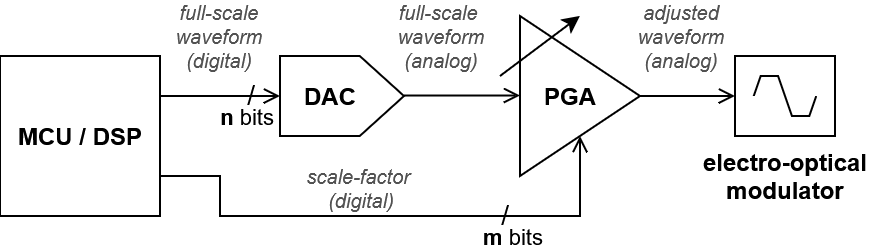
\includegraphics[width=0.48\textwidth]{img/dedicated_gain_stage.png}
    \caption{Modulator with a dedicated analog gain stage. MCU/DSP outputs a fixed--scale digital waveform, which directly drives a DAC. Then, before reaching the electro--optic actuator, the scale factor is adjusted with a programmable gain amplifier (PGA), or a custom analog gain stage, resulting in adjusted--scale waveform. }
    \label{fig:dedicated_gain_stage}
\end{figure}

\noindent
In this configuration DAC and PGA are driven with $n-$ and $m$--bit words. The digital nature of controlling gain stage introduces unavoidable quantization noise into the control loop. However, one of the important advantages of this setup is the intrinsic separation of the modulation problem into two smaller parts - generating the waveform in fixed--scale and applying the scale factor afterwards. The two can be implemented by software without dependence on each other, resulting in two distinct control loops. On the contrary, the dedicated gain stage is a subject to interferences. It may have its own nonlinearities and introduce delay in the signal path. Most importantly, its bandwidth may be gain dependent, distorting the waveform.

% FIX FIX FIX
% Utilizing the observation, that the scale factor shall not vary by more than a few per cent during the device's lifetime, it can be assumed that if the PGA was driven by $n+1$ bits, the performance would not be affected.
% Voltage range would have to be set for the worst--case scenario plus some margin, to always be sufficient. Full scale wouldn't be used most of the time. Even if the scale factor was to drop to 50\% of the available range, which is beyond any pessimistic scenario, the overall performance would remain no worse than when using a $n$--bit control. From this an all--digital architecture can be defined.

\subsection{All-digital approach - software--defined solution}
The all--digital approach depicted in Figure~\ref{fig:all_digital} utilizes the availability and wide range of high precision digital--to--analog converters. It allows for disposing the physical gain stage, by applying scale factor digitally, prior to driving the DAC. This requires DAC reference voltage to be high enough to cover all possible ranges. This approach also introduces quantization noise. These two disadvantages, are similarily the problems of the previous solution. The main advantage this idea brings is the minimization of the amount of electronic components used. This yields less sources of potential nonlinearities and electromagnetic interference. Since the electro--optic modulator has high input impedance, the output of a voltage--DAC can be directly connected to it, omitting any buffers on the signal path. The profit resulting from less noisy electronics copensate the unavoidable DAC resolution loss - its full range may never be utilized because of the required margins. Moreover, the following sections discusses an algorithmic approach, which regains one bit of accuracy, when using the all--digital architecture.

\begin{figure}[ht]
    \centering
    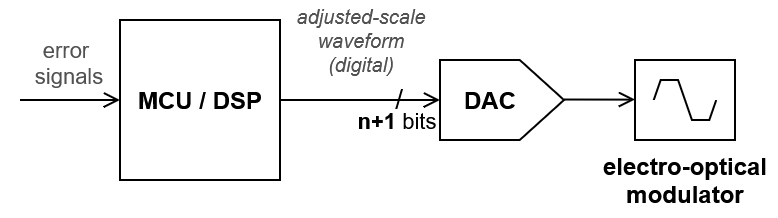
\includegraphics[width=0.48\textwidth]{img/all_digital.png}
    \caption{All--digital modulator consists of minimal number of electronic components. In some cases this can simply be a DAC alone.}
    \label{fig:all_digital}
\end{figure}

\noindent
Additional advantage of leaning towards the proposed architecture is that the whole design becomes a software--defined solution. As in other fields, such approach brings flexibility from the R\&D process perspective. This is mainly because, while iterating hardware is a time--consuming process, updating software is relatively quick and cost effective. Moving the problem completely to the software side obviously makes the implementation more complex, but at the same time it limits the amount of interaction at the boundary of software and hardware development, significantly reducing overhead. From this perspective the net workload remains relatively stable, offering slightly different - more modern - approach.

\subsubsection{Voltage reference}
For the all--digital modulator an adequate reference voltage has to be set up to account for the maximum possible scale factor in the devices lifetime. From Equation~\ref{eq:bias_order} it results, that a span of $1.5\pi$ is required for biasing and additionally, the Serrodyne modulator requires a span of $2\pi$. This yields a required span of $S = 3.5\pi$. Minimum DAC reference $V_{ref}^{min}$ shall account for it with some margin $M \in [1.0; 1.1]$:

\begin{equation}
    V_{\text{ref}}^{\text{min}} = V_{\pi}^{\text{max}} \cdot S \cdot M
    \label{eq:minimum_reference_voltage}
\end{equation}

\noindent
The $V_{\pi}^{\text{max}}$ denotes the highest expected half--wave voltage. When determining final reference voltage it is advantageous to round it up to a multiple of one of typically available chip references (Equation~\ref{eq:reference_voltage_ceil}), e.g. $K \times 5V$ or $K \times 4.096V$. It makes implementing the elctronic circuit more straightfroward. In practice, a fair compromise is to utilize the resulting voltage excess for the margin $M$, so that after adding it, the $V_{ref} \approx V_{ref}^{min}$.

\begin{equation}
    V_{\text{ref}} = \lceil V_{\text{ref}}^{\text{min}} \rceil
    \label{eq:reference_voltage_ceil}
\end{equation}

\subsubsection{Drive accuracy and quantization error}
Usage of a DAC results in quantization error. Converter resolution $N$ and its reference voltage determine the minimal controllable voltage change as

\begin{equation}
    \Delta{}v = V_{\text{ref}} \cdot 2^{-N}
    \label{eq:dac_voltage_resolution}
\end{equation}

\noindent
In phase domain the scale factor can be thus controlled with the accuracy corresponding to $\Delta{}v$ relative to the actual scale factor:
% FIX FIX FIX
% Scale factor error results from the distance between its controlled and actual values. It corresponds to half of $\Delta{}v$. It can vary in time, as the actual $V_{\pi}$ may continously change over time, but rather slowly (compared to the possible modulation frequencies).

\begin{equation}
    \Delta\phi_{v} = \frac{\Delta{}v}{V_\pi}
    \label{eq:relative_scale_factor_error}
\end{equation}

\noindent
Due to the linear scale--factor dependence it will slowly vary over time, but its magnitude shall remain stable, as the drift is expected to only be at the level of percents. By substituting previous formulas, the final control accuracy and quantization error are:

\begin{equation}
    \begin{split}
        \Delta\phi_{v} & = \frac{\lceil V_{\pi}^{\text{max}} \cdot S \cdot M \rceil \cdot 2^{-N}}{V_{\pi}} \\
        \Delta\phi_{q} & = \frac{1}{2} \cdot \Delta\phi_{v}
    \end{split}
    \label{eq:error}
\end{equation}

\noindent
Exemplary calculation, based on real--world values yields:

\begin{equation}
    \begin{split}
        \Delta\phi_{v}^{\text{ex}} & = \frac{\lceil \overbrace{4.5V}^{V_{\pi}^{\text{max}}} \cdot \overbrace{3.5}^{S} \cdot \overbrace{1.025}^{M} \rceil \cdot \overbrace{2^{-16}}^{2^{-N}} }{\underbrace{3.5V}_{V_{\pi}}} = \\
                                   & = \frac{\lceil 16.14V \rceil \cdot 2^{-16}}{3.5V} = \frac{\overbrace{16.384V}^{4 \cdot 4.096V} \cdot 2^{-16}}{3.5V} =                                                                   \\[10pt]
                                   & = 2^{-16} \cdot 4.68 = 2^{-16} \cdot 2^{2.23}                                                                                                                                           \\[10pt]
        \Delta\phi_{q}^{\text{ex}} & = \frac{1}{2} \cdot \Delta\phi_{v}^{\text{ex}} = 2^{-16} \cdot 2^{1.23}
    \end{split}
    \label{eq:error_example}
\end{equation}

\noindent
From this it is clear, that the quantization error, bound to controllable resolution can be improved by selecting a converter with greater number of bits.
However, any selected resolution will always be a subject to losing just over two bits. It must be noted, that most of this loss is due to the span $S$, required for proper operation of the algorithm. It is not a consequence of using the proposed all--digital architecture. The quantization error follows the achieved accuracy. In each of the bias points, the following drive levels are possible:

\begin{equation}
    \begin{split}
        \phi_{4n+0}^{+\frac{3}{2}\pi} & = k_{4n+0} \cdot \Delta\phi_{v} = +\frac{3}{4}\pi + \delta_{4n+0} \\
        \phi_{4n+0}^{-\frac{1}{2}\pi} & = k_{4n+1} \cdot \Delta\phi_{v} = -\frac{1}{4}\pi - \delta_{4n+1} \\
        \phi_{4n+0}^{-\frac{3}{2}\pi} & = k_{4n+2} \cdot \Delta\phi_{v} = -\frac{3}{4}\pi - \delta_{4n+2} \\
        \phi_{4n+0}^{+\frac{1}{2}\pi} & = k_{4n+3} \cdot \Delta\phi_{v} = +\frac{1}{4}\pi + \delta_{4n+3}
    \end{split}
    \label{eq:22213}
\end{equation}

\noindent
Value $k \in [-2^{N-1}, 2^{N-1}-1)$ is an integer, in range of the used DAC (of $N$ resolution). By incrementing/decrementing $k_{n}$ the error $\delta_{n}$ can be controlled with the resolution of $\Delta\phi_{v}$. However, because of the quantization error, its value can always be up to $\Delta\phi_{q}$.

% TODO number of bits n change to uppercase N (& M)
% TODO error floor
% TODO this paper does not focus on serrodyne precision, only on scale factor accuracy

\section{Precision estimation and impact}
To close the scale factor control loop, a feedback is required. It is calculated from the difference of incident light intensity between two consecutive bias points. The total phase difference $\Delta\phi_{k}$, affecting intensity for the sample $k$, results from the current drive $\phi_k$ and the drive two points prior:

\begin{equation}
    \Delta\phi_{n} = (\phi_{n} - \phi_{n-2}) + \underbrace{\Delta\phi_{s, n} + \Delta\phi_{r, n}}_{=0}
    \label{eq:phase_shift_difference}
\end{equation}

\noindent
The values of $\Delta\phi_{s, n}$ and $\Delta\phi_{r, n}$ denote Sagnac--induced and nulling ramp shifts - assumed to be zero for this analysis. By using equations \ref{eq:response} and \ref{eq:bias_order} and assuming the $cos$ function linear near the bias points (Equation~\ref{eq:cosine_linearization}), intensity values at each point are:

% TODO emphasize at the beginning thast this focuses of scale factor control, not rotation calculation, thus it is assumed that rotation is zero for the analysis

\begin{equation}
    \begin{split}
        P_{4n+0}^{+\frac{3}{2}\pi} & = \frac{P_0}{2} \cdot (1 + cos(\Delta\phi_{4n+0}^{+\frac{3}{2}\pi})) =                                                                                                                          \\
                                   & = \frac{P_0}{2} \cdot (1 + cos(\underbrace{\phi_{4n+0}^{+\frac{3}{2}\pi}}_{\frac{3}{4}\pi + \delta_{4n+0}} - \underbrace{\phi_{4n-2}^{-\frac{3}{2}\pi}}_{-(\frac{3}{4}\pi + \delta_{4n-2})})) = \\
        %  & \enspace = \frac{P_0}{2} \cdot (1 + cos(() - ())) = \\
                                   & = \frac{P_0}{2} \cdot (1 + cos(\frac{3}{2}\pi + \delta_{4n+0} + \delta_{4n-2})) =                                                                                                               \\
                                   & = \frac{P_0}{2} \cdot (1 + (\delta_{4n+0} + \delta_{4n-2}))                                                                                                                                     \\[10pt]
        P_{4n+1}^{-\frac{1}{2}\pi} & = \frac{P_0}{2} \cdot (1 - (\delta_{4n+1} + \delta_{4n-1}))                                                                                                                                     \\
        P_{4n+2}^{-\frac{3}{2}\pi} & = \frac{P_0}{2} \cdot (1 + (\delta_{4n+2} + \delta_{4n+0}))                                                                                                                                     \\
        P_{4n+3}^{+\frac{1}{2}\pi} & = \frac{P_0}{2} \cdot (1 - (\delta_{4n+3} + \delta_{4n+1}))
    \end{split}
    \label{eq:incident_power}
\end{equation}

\begin{equation}
    \begin{split}
        cos(\phi_{b} + \Delta\phi) & = \underbrace{cos(\phi_{b})}_{=0} + cos'(\phi_{b}) \cdot \Delta\phi =   \\
                                   & = -sin(\phi_{b}) \cdot \Delta\phi                                       \\
        \text{for } \phi_{b} \in   & \{+\frac{3}{2}\pi, +\frac{1}{2}\pi, -\frac{1}{2}\pi, -\frac{3}{2}\pi\}
    \end{split}
    \label{eq:cosine_linearization}
\end{equation}

\noindent
Feedback signal calculated at samples $4n+1$ and $4n+3$ is:

\begin{equation}
    \begin{split}
        e_{4n+1}^{-\frac{1}{2}\pi} & = P_{4n+1}^{-\frac{1}{2}\pi} - P_{4n+0}^{+\frac{3}{2}\pi} =                            \\ 
                                   & = -\frac{P_0}{2} \cdot (\delta_{4n+1} + \delta_{4n+0} + \delta_{4n-1} + \delta_{4n-2}) \\
        e_{4n+3}^{+\frac{1}{2}\pi} & = P_{4n+3}^{+\frac{1}{2}\pi} - P_{4n+2}^{-\frac{3}{2}\pi}  =                           \\
                                   & = -\frac{P_0}{2} \cdot (\delta_{4n+3} + \delta_{4n+2} + \delta_{4n+1} + \delta_{4n+0}) \\
    \end{split}
    \label{eq:difference}
\end{equation}

\noindent
It can be generalized for every odd bias sample, where it shall be calculated - this results from the demodulation algorithm assumptions \cite{lefevre1993fiber}:

\begin{equation}
    e_{2n+1} = -\frac{P_0}{2} \cdot (\underbrace{\delta_{2n+1}}_{\text{current}} + \underbrace{\delta_{2n+0} + \delta_{2n-1} + \delta_{2n-2}}_{\text{three prevoius errors}})
    \label{eq:difference_generic}
\end{equation}

\noindent
The feedback signal, used for loop closure, is dependent on four recent drive values. Because the DAC can be controlled with $\Delta{}v$ resulotion, the scale factor error, and thus the occuring errors $\delta_n$ are all controllable with a fixed delta of $\Delta\phi_{v}$ corresponding to $\Delta{}v$. In particular the presented error $e_{2n+1}$ for the last four samples can be controlled with $\Delta\phi_{v}$ accuracy, but this may only happen when the current sample accounts for the three previous ones.

\section{Algorithm design}
From the derived error equation a few important results can be determined. In this section - firstly - the most likely mistakes in algorithm design are emphasized. Then - secondly - a correct modulator implementation is presented in pseudocode.

\subsection{Naive implementation}
\subsubsection{Number of samples considered}
Modulation algorithm is a subsystem for the contol loop implemented in the device. Given the fact that the scale factor feedback signal is obtained by comparing two consecutive intensity levels (Equation~\ref{eq:difference}), an intuitive conclusion follows, that the control loop shall operate at the rate corresponding to the period of two samples. While being correct, this assumption requires additional constraints, otherwise it leads to a naive and incorrect solution. From Equation~\ref{eq:difference_generic} it is clear, that the feedback signal depends on four adjacent samples, not two. Without the conducted derivation this would not be immediately obvious. A naive algorithm, only considering one sample pair could easily lead to control loop oscillations and performance degradation. A correct solution is to always account for the recent two drive values, when calculating the next two. 

\subsubsection{Drive symmetry}
The intended drive values between samples $n$ and $n+2$ are symmetrical, i.e. they differ in sign, but have identical amplitude. However, for an actual signal driven with a DAC, this assumption falls short. This is due to the discrete nature of a DAC. In ideal scenario a symmetric drive would be desired, but this assumes perfectly controlled amplitude. When the amplitude is discreticized, the most reasonable solution is to utilize as much of the resolution, while keeping the drive signals relatively symmetrical - as a second priority. This allows for having a $1 [lsb]$ amplitude difference, which results in phase shift control accuracy of a single lsb. Otherwise, the effective resolution would be lowered by one bit - the difference betweeen two effective drive values would correspond to $(k_{n} \cdot \Delta\phi_{v}) - (-k_{n} \cdot \Delta\phi_{v}) = 2\Delta\phi_{v}$ for adjacent $k_{n}$, while the DAC offers control resolution of a single $\Delta\phi_{v}$.

\subsubsection{Rounding factor}
Another designing corner cut is the rounding method selection for driving discrete DAC values while performing calculations with fractional resolution. Especially prone designs are the ones using floating point arithmetics (e.g. IEEE-754 float/double, typically used in C/C++ of programmable logic). The problem lays in the rounding direction when working with both positive and negative values (which is the case for driving bias points both ways from zero). Mathematicall symmetry of this operation leads to resolution loss. This is regardless of whether the selected rounding algorithm is:
\begin{itemize}
    \item truncation, or rounding towards zero ($-2.2 \rightarrow -2$, $2.7 \rightarrow 2$),
    \item mathematical rounding ($2.4 \rightarrow 2$, $2.5 \rightarrow 3$),
    \item rounding away from zero ($-2.4 \rightarrow -3$, $2.4 \rightarrow 3$),
\end{itemize}

\noindent
\textbf{TODO check example for all three!!! TODO}

\noindent
If the algorithm rounds fractional values symmetrically, it will lead to the same resolution degradation as described in the previous section. While the effect is the same, the reason is different as the algorithm may not necessarily be implemented to use fractional arithmetics - even though it would rather be recommended. This case is worth of emphasizing, as multiple implementations are expected to be using floating point arithmetics in particular. This important nummerical issue arises when performing calculations in floating point and simply mapping the result to binary or U2 format required by a DAC. The following snippet shows an example.

\begin{figure}[ht]
    \centering
    {\scriptsize\begin{verbatim}
// intended half-wave voltage in DAC units [lsb]
uint8_t scaleFactor = 14u; 

// calculated DAC drive values
int8_t dac[4n+0] = scaleFactor *  0.75 =  10.5 =>  11;
int8_t dac[4n+1] = scaleFactor * -0.25 = -3.5  =>  -4;
int8_t dac[4n+2] = scaleFactor * -0.75 = -10.5 => -11;
int8_t dac[4n+3] = scaleFactor *  0.75 =  3.5  =>   4;
    \end{verbatim}}
    \caption{Example of the possible difference between the intended and actual drive values in the context of applying mathematical rounding method.}
    \label{fig:snippet_rounding}
\end{figure}

\textbf{TODO LABELS CORRECT}

\noindent
In effect the resulting drive does not always correspond to the intended difference, even though it is calculated in $\Delta\phi_{v}$ domain. In the presented example the result is $30$ while the intended scale factor indicates it shall be $28$ (effective difference for Equation~\ref{eq:difference_generic}):

\begin{equation}
    \begin{split}
        ((4) - (-4)) - ((-11) - (11))         & = 30 \quad [\Delta\phi_{v}] \\
        ((3.5) - (-3.5)) - ((-10.5) - (10.5)) & = 28 \quad [\Delta\phi_{v}]
    \end{split}
\end{equation}

Additional problem is that this only happens at the level of the least significant bit, so the only reasonable way to track this error is through nummerical analysis or simulation of the actual algorithm. It will not be visible in operation, due to the error magnitude relative to the rest of the waveform.

\textbf{TODO TODO screen z SDK? TODO}

\subsection{Optimal implementation}
Correct implementation, presented in the snippet in Figure~\ref{fig:snippet_implementation}, accomodates for the mentioned traps. It controls four recent samples at all times and it selects a rounding method, which has two advantages. Firstly, it is correct in terms of modulating with the accuracy of a single lsb. Secondly, it is implementation efficient. It utilizes the property of U2 representation, which always rounds values towards $-\inf$, resembling mathematical $floor$ operation.
It also uses fixed--point arithmetics to perform calculations with fractional precision. The format used is Q6.2, where the values $\pm\frac{1}{4}$ and $\pm\frac{3}{4}$ are simply expressed as integers $\pm1$ and $\pm3$. For the final result the fractional bits are simply dropped - using right--shift operation in this case. It has to be noted, that fixed--point arithmetics is an optimal choice for implementing an algorithm which does not deal with values high dynamic range and where determinismregarding accuracy is of paramount importance. Moreover, a floating--point format will also utilize more resources - both in the context of performing operations (addition, multiplication, etc.) and also for value storage (they require additional bits for storing both mantissa and exponent). 

\begin{figure}[ht]
    \centering
    {\scriptsize\begin{verbatim}
{ // two previous (already driven) bias points [4n-2, 4n-1]
uint8_t scaleFactor[4n-2] = 13;

int8_t dac[4n-2] = (scaleFactor[4n-2] *  0x3) >> 2 = 9;
int8_t dac[4n-1] = (scaleFactor[4n-2] * -0x1) >> 2 = -4;
}

{ // two current (to be driven) bias points [4n+0, 4n+1]
uint8_t scaleFactorIntended[4n+0] = 14u;
uint8_t scaleFactor[4n+0] = 
    (2 * scaleFactorIntended[4n+0]) - scaleFactor[4n-2];

int8_t dac[4n+0] = (scaleFactor[4n+0] * -0x3) >> 2 = -12;
int8_t dac[4n+1] = (scaleFactor[4n+0] *  0x1) >> 2 = 3;
}
    \end{verbatim}}
    \caption{Pseudocode for controlling the scale factor for the current two bias points while accounting for the values driven previously. The arithmetics is implemented using Q6.2 fixed--point format. Rounding towards $-\inf$ is natively handled for this format.}
    \label{fig:snippet_implementation}
\end{figure}

In this case the effective drive corresponds to the scale factor, which was intended for the latter two bias points, but it had to account for the previous pair:

\begin{equation}
    ((3) - (-4)) - ((-12) - (9)) = 28 \quad [\Delta\phi_{v}]
\end{equation}

Another possible implementation is to simply execute the control loop once every four samples. This results in very straightforward implementation, which apriori determines all four drive levels and applies them. however, an important drawback of such solution is that only two of four bias points from Equation~\ref{eq:bias_order} are usable for both scale factor and rotation calculation. This results from the dependence of the rotation measurement accuracy on scale factor in each of the bias points. A detailed analysis in that matter is a subject for further work. 

\section{Conclusions and further work}
This work discusses certain aspects of implementing a modulator for closed--loop iFOGs, which are of crucial importance when thinking of a modern design. An all--digital hardware architecture was presented and advocated for, as it has the greatest potential for performance improvements. What follows are some software development challenges, some of which were presented. Solutions have been provided for those and an algorithm base was established, however this work requires continuation. This is especially valid for the mathematical analysis conducted in this paper, which also has to be done for rotation calculation - in particular, the effect of generating a ramp signal with Serrodyne modulation - intentionally omitted at this time. Furthermore, a complete analysis including demodulation process and control loops closure needs to be provided to ensure the whole design is well optimized - because the system is as performant, as its least performing element.

\noindent
This paper provides background for further optimizations in software devlopment for the closed--loop iFOG. 

\textbf{TODO TODO TODO}
% what can you add?
% what would you change?
% rewrite the conclusions section
% what respected scientiic paper could be cited here?
% check indentation
% check grammatically
% check interpunction
% prpose changes to make it more readable, to make the user "flow" through the content

% review against general rules of writitng a scientific paper
% review against the rules in original.tex


\begin{thebibliography}{00}
    \bibitem{post1967sagnac} Post, Evert Jan. "Sagnac effect." Reviews of Modern Physics 39.2 (1967): 475.
    \bibitem{sagnac1913ether} Sagnac, Georges. "L'éther lumineux démontré par l'effet du vent relatif d'éther dans un interféromètre en rotation uniforme." CR Acad. Sci. 157 (1913): 708-710.
    \bibitem{pavlath1996closed} Pavlath, George A. "Closed-loop fiber optic gyros." Fiber Optic Gyros: 20th Anniversary Conference. Vol. 2837. SPIE, 1996.
    \bibitem{babu2016digital} Babu, G. Harish, A. Venkata Anuhya, and N. Venkatram. "Digital signal processing scheme for open loop and closed loop IFOG using MATLAB/SIMULINK." Indian Journal of Science and Technology 9.11 (2016): 1-10.
    \bibitem{lefevre1993fiber} Lefevre, Herve C. "Fiber optic gyroscopes." Optical Fiber Sensors. Dordrecht: Springer Netherlands, 1993.
    \bibitem{wang2012method} Wang, Wei, Junlong Wang, and Zhengxin Zhao. "Method to control the gain in modulation chain of closed-loop fiber optic gyroscope with periodical biasing modulation." Optical Engineering 51.6 (2012): 064401-064401.
    \bibitem{salvestrini2011analysis} Salvestrini, Jean Paul, et al. "Analysis and control of the dc drift in linbo3-based mach–zehnder modulators." Journal of lightwave technology 29.10 (2011): 1522-1534.
    \bibitem{ulversoy2010software} Ulversoy, Tore. "Software defined radio: Challenges and opportunities." IEEE Communications Surveys \& Tutorials 12.4 (2010): 531-550.
    \bibitem{liu2022impact} Liu, Zongwei, Wang Zhang, and Fuquan Zhao. "Impact, challenges and prospect of software-defined vehicles." Automotive Innovation 5.2 (2022): 180-194.
    
\end{thebibliography}
\end{document}
